\chapter{Vorbereitung}
\begin{equation}
  h_{k}(n)=\sigma(n)*(cos(k(n+1)\frac{2*\pi}{N})+jsin(k(n+1)\frac{2*\pi}{N}=h_{k}^{RE}(n)+jh_{k}^{IM}(n)
\end{equation}
Ergebnis der rechtsseitigen z-Transformation.\\
Imaginärteil:
\begin{equation}
  X_{R_{sin}}(z)= \frac{z^{2}*sin(\frac{\pi}{N}*k)}{z^{2}-2*cos(\frac{\pi}{N}*k)*z+1}
\end{equation}
Realteil:
\begin{equation}
  X_{R_{cos}}(z)=\frac{z^{2}*cos(\frac{\pi}{N}*k)-z}{z^{2}-2*cos(\frac{\pi}{N}*k)*z+1}
\end{equation}
\begin{figure}[H]
  \centering
    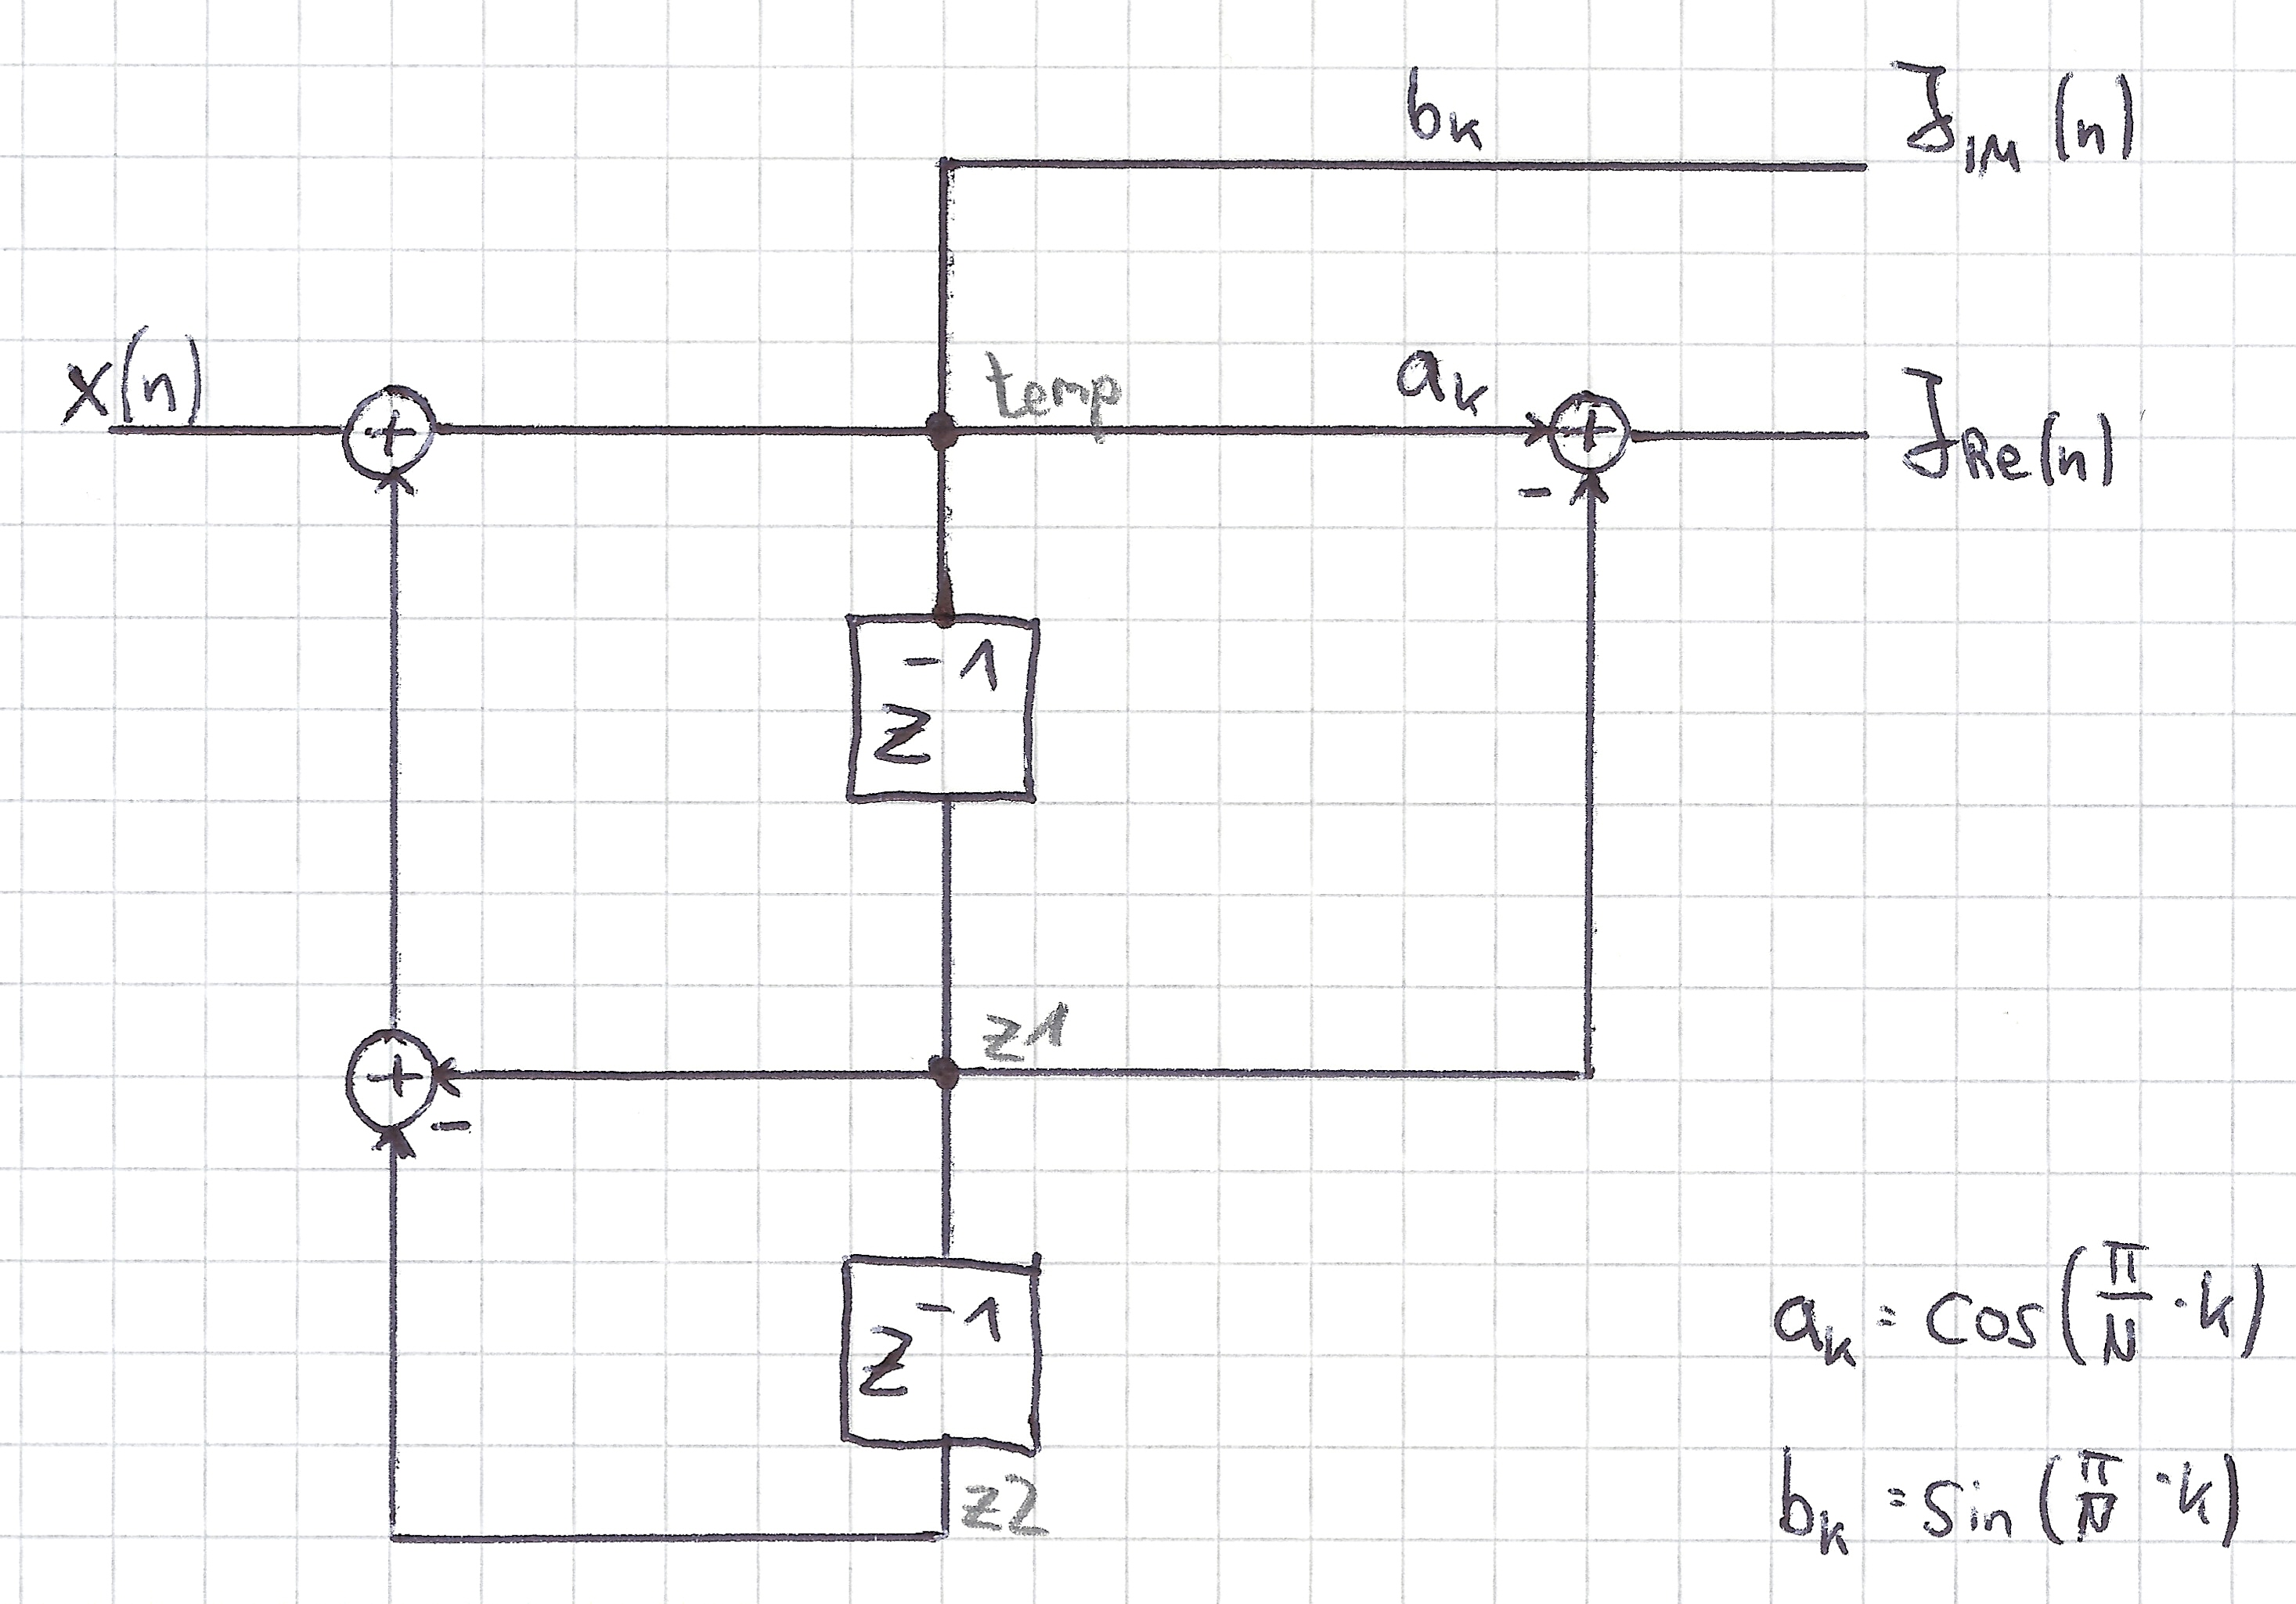
\includegraphics[width=\textwidth]{KDFII0001.jpg}
  \caption{Kanonische Direktform 2 des Filters}
  \label{fig:KDFII}
\end{figure}